\documentclass[final,xcolor={dvipsnames,svgnames,x11names,table}]{beamer}
\usetheme{RJH}
%\usetheme{Boadilla}
\usepackage[orientation=portrait,size=a0,scale=1.3]{beamerposter}
% \usepackage[orientation=portrait, size=custom, width=84.1, height=118.9, scale=1]{beamerposter}
\usepackage[absolute,overlay]{textpos}
\usepackage{pifont}
\usepackage{ulem}
\usepackage{bm}
\usepackage{siunitx}
\usepackage[export]{adjustbox}
\usepackage{gmp}
\usepackage{smartdiagram}
\usesmartdiagramlibrary{additions}
\usepackage{booktabs}
%\usepackage{enumitem}

%\DeclareGraphicsRule{.1}{mps}{*}{}

\usepackage[listings,theorems]{tcolorbox}


\usepackage{libertine}
\setlength{\TPHorizModule}{1cm}
\setlength{\TPVertModule}{1cm}

\usepackage{tikz,tikz-3dplot} %nalipour
\usetikzlibrary{shapes,arrows, decorations.pathreplacing}%, snakes} %nalipour

\def\Put(#1,#2)#3{\leavevmode\makebox(0,0){\put(#1,#2){#3}}}

% Raised Rule Command:
%  Arg 1 (Optional) - How high to raise the rule
%  Arg 2            - Thickness of the rule
\newcommand{\raisedrule}[2][0em]{\leaders\hbox{\rule[#1]{1pt}{#2}}\hspace{13.5cm}}

\newcommand{\dotrule}[1]{%
   \parbox[]{#1}{\dotfill}}

\setbeamertemplate{bibliography entry title}{}
\setbeamertemplate{bibliography entry location}{}
\setbeamertemplate{bibliography entry note}{}
\footer{}


% \usebackgroundtemplate{%%\includegraphics[width=\paperwidth]{Figures/CLIC_canvas_accelerator_small.jpg}}


\title{\Huge{Design of a drift chamber tracking system for the IDEA experiment at FCC-ee}}
\author{\vspace*{1.5cm}{\Large{Niloufar Alipour Tehrani (CERN), Benedikt Hegner, Giovanni Francesco Tassielli, Francesco Grancagnolo}\\\vspace*{1cm}{\Large{2018 IEEE Nuclear Science Symposium and Medical Imaging Conference, Sydney, Australia}}}}
% \footer{}
\institute{CERN}
\date{}
%\footimage{}

% \usepackage[backend=bibtex,style=numeric-comp,firstinits=true]{biblatex}
% \bibliography{bib}
% \setbeamertemplate{bibliography item}[text]
% \renewcommand*{\bibfont}{\footnotesize}

% tcolorbox styles
\tcbset{%
    noparskip,
    colback=white, %background color of the box
    colframe=i6colorblockbg, %color of frame and title background
    coltext=black, %color of body text
    coltitle=white, %color of title text
    fonttitle=\bfseries,
    alerted/.style={coltitle=red,
                     colframe=gray!40},
    subtcolorbox/.style={coltitle=black,
                     colframe=i6colorscheme3,
                     colback=white,
                     coltitle=i6colorblockbg},
    }


\begin{document}
\begin{frame}

\begin{textblock}{2}(0.8,0.25)

\includegraphics[width=4.\textwidth]{Figures/logo_cern.pdf}
\end{textblock}
\begin{textblock}{6}(71,0.25)

\includegraphics[width=1.5\textwidth]{Figures/FCC-logo}
\end{textblock}
\begin{textblock}{20}(4.5, 11)
%\textcolor{red}{\small{\url{http://clicdp.web.cern.ch/}}}
\end{textblock}


%%%%%%%%%%%%%%%%%%%%%%%%%%%%%%%%%%%%%
%%%                             Block                                %%%
%%%%%%%%%%%%%%%%%%%%%%%%%%%%%%%%%%%%%
\begin{textblock}{40}(0.5, 14)
  \begin{tcolorbox}[title=The Future Circular Collider Experiment (FCC)]

  \begin{columns}
    \column{0.5\textwidth}
      \begin{itemize}
        \item A future possibility for the post-LHC era
        \item 3 options of circular colliders
          \begin{itemize}
            \item FCC-ee: electron - positron collisions
            \item FCC-hh: proton - proton collisions
            \item FCC-eh: electron - proton collisions
          \end{itemize}
        \item $\sim$100~km tunnel in Geneva area
        \item FCC-ee collider parameters:
      \end{itemize}
        \centering
      	\begin{tabular}{l c c c c}
        	\toprule
      	   Stages & Z & WW & H (ZH) & t\={t} \\
      	   \midrule
           Beam energy [GeV] & 45.6 & 80 & 120 & 182.5 \\
           Average bunch spacing [ns] & 19.6 & 163 & 994 & 3396\\
      	   \bottomrule
      	\end{tabular}

    \column{0.5\textwidth}
      \centering
      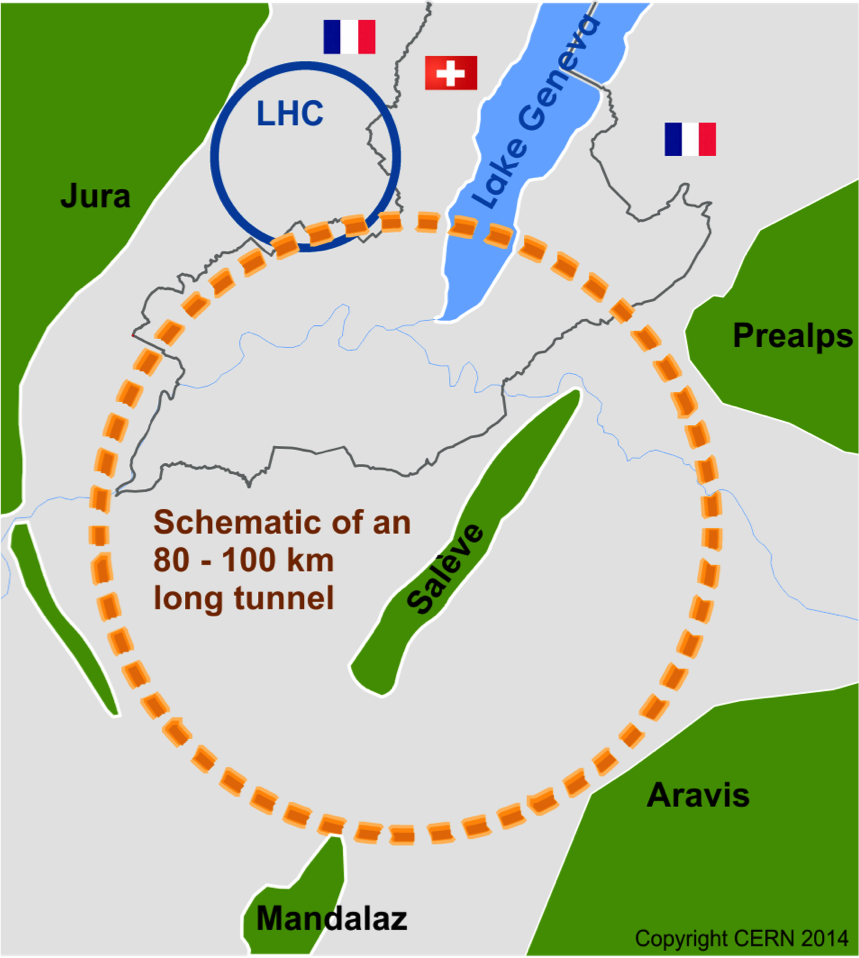
\includegraphics[width=0.9\textwidth]{Figures/cernFCC}
  \end{columns}

  \end{tcolorbox}
\end{textblock}

% %%%%%%%%%%%%%%%%%%%%%%%%%%%%%%%%%%%%%
% %%%                             Block                 %%%
% %%%%%%%%%%%%%%%%%%%%%%%%%%%%%%%%%%%%%
\begin{textblock}{40}(41, 14)
  \begin{tcolorbox}[title=FCCSW: Physics and Detector simulations with FCCSW]

  \begin{itemize}
    \item Common software for all FCC experiments (ee, hh \& eh)
    \item Detector and physics studies
      \begin{itemize}
        \item Fast \& full simulations
        \item One software stack from event generation to physics analysis
      \end{itemize}
    \item Collaborative approach with other CERN experiments
      \begin{itemize}
        \item Gaudi from LHC
        \item DD4hep from CLIC \& LHCb
        \item New solutions where needed
      \end{itemize}

  \end{itemize}



  \vspace{1cm}

  \centering
   % \scalebox{2}{
  	 \smartdiagramset{back arrow disabled=true, module minimum width=4cm, text width=4cm, module minimum height=2cm, module x sep=6cm}
  	 	\smartdiagram[flow diagram:horizontal]
  	 	{%
  	   	{Geometry\\DDhep}, Segmentation, {Geant4 \\simulation}, Digitization%
  	 	}
     % }
  \end{tcolorbox}
\end{textblock}

% %%%%%%%%%%%%%%%%%%%%%%%%%%%%%%%%%%%%%
% %%%                             Block                                %%%
% %%%%%%%%%%%%%%%%%%%%%%%%%%%%%%%%%%%%%
\begin{textblock}{40}(0.5, 36)
  \begin{tcolorbox}[title=The IDEA detector concept for FCC-ee]

  \begin{columns}
    \column{0.5\textwidth}
      \begin{itemize}
        \item Two detector concepts for the FCC-ee collider
          \begin{enumerate}
            \item The IDEA detector concept (focus of this poster)
            \item A CLIC-based (silicon-based) detector
          \end{enumerate}
        \item Ultimate goal for the IDEA detector concept
          \begin{itemize}
            \item Vertex detector: MAPS
            \item Ultra-light drift chamber with particle identification
            \item Double readout calorimetry
            \item Aditional silicon disk layers placed in the space between the drift chamber and the dual readout calorimeter to increase the forward coverage
            \item 2~T solenoidal magnetic field
            \item Instrumented return yoke
            \item Large tracking volume (R $\sim$ 8~m) for very weakly coupled (long-lived) particles
          \end{itemize}
      \end{itemize}


    \column{0.5\textwidth}
      \centering
      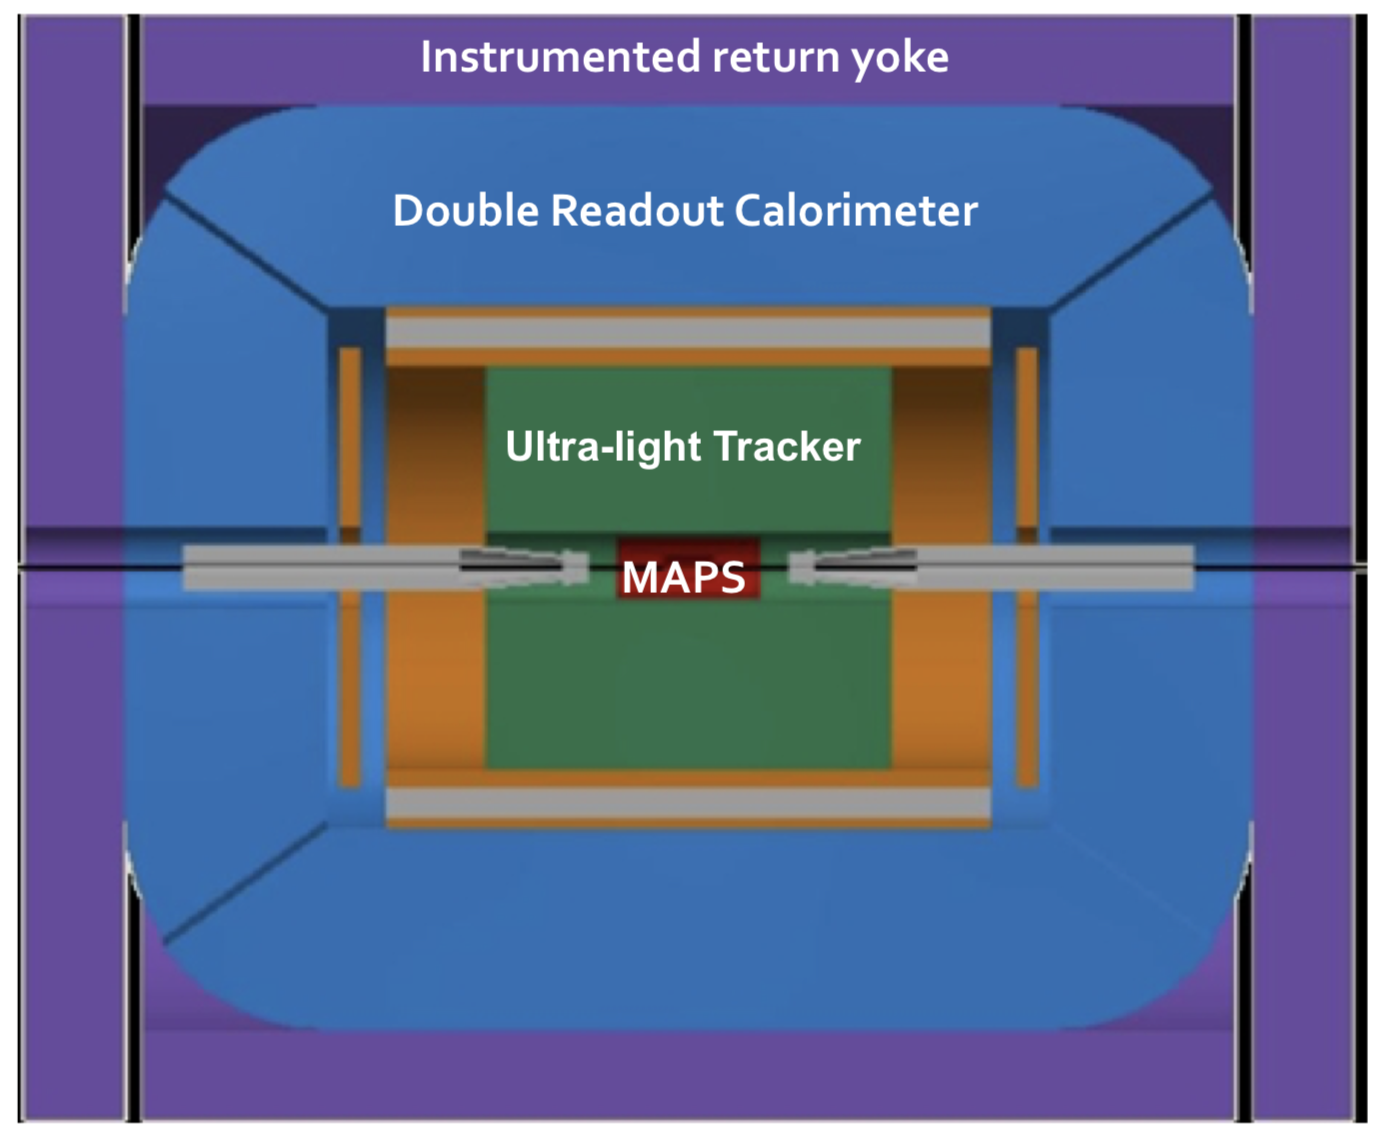
\includegraphics[width=\textwidth]{../figures/FCCeeIDEAConcept}
  \end{columns}


  \end{tcolorbox}
\end{textblock}

%%%%%%%%%%%%%%%%%%%%%%%%%%%%%%%%%%%%%
%%%                             Block                                %%%
%%%%%%%%%%%%%%%%%%%%%%%%%%%%%%%%%%%%%
\begin{textblock}{40}(41, 30)
  \begin{tcolorbox}[title=Simulation of the drift chamber within FCCSW]

  \begin{itemize}
    \item The IDEA detector as simulated with FCCSW
  \end{itemize}
  % \begin{columns}
  % \column{0.5\textwidth}
  \begin{tikzpicture}
    \node[anchor=south west,inner sep=0] (image) at
    (0,0){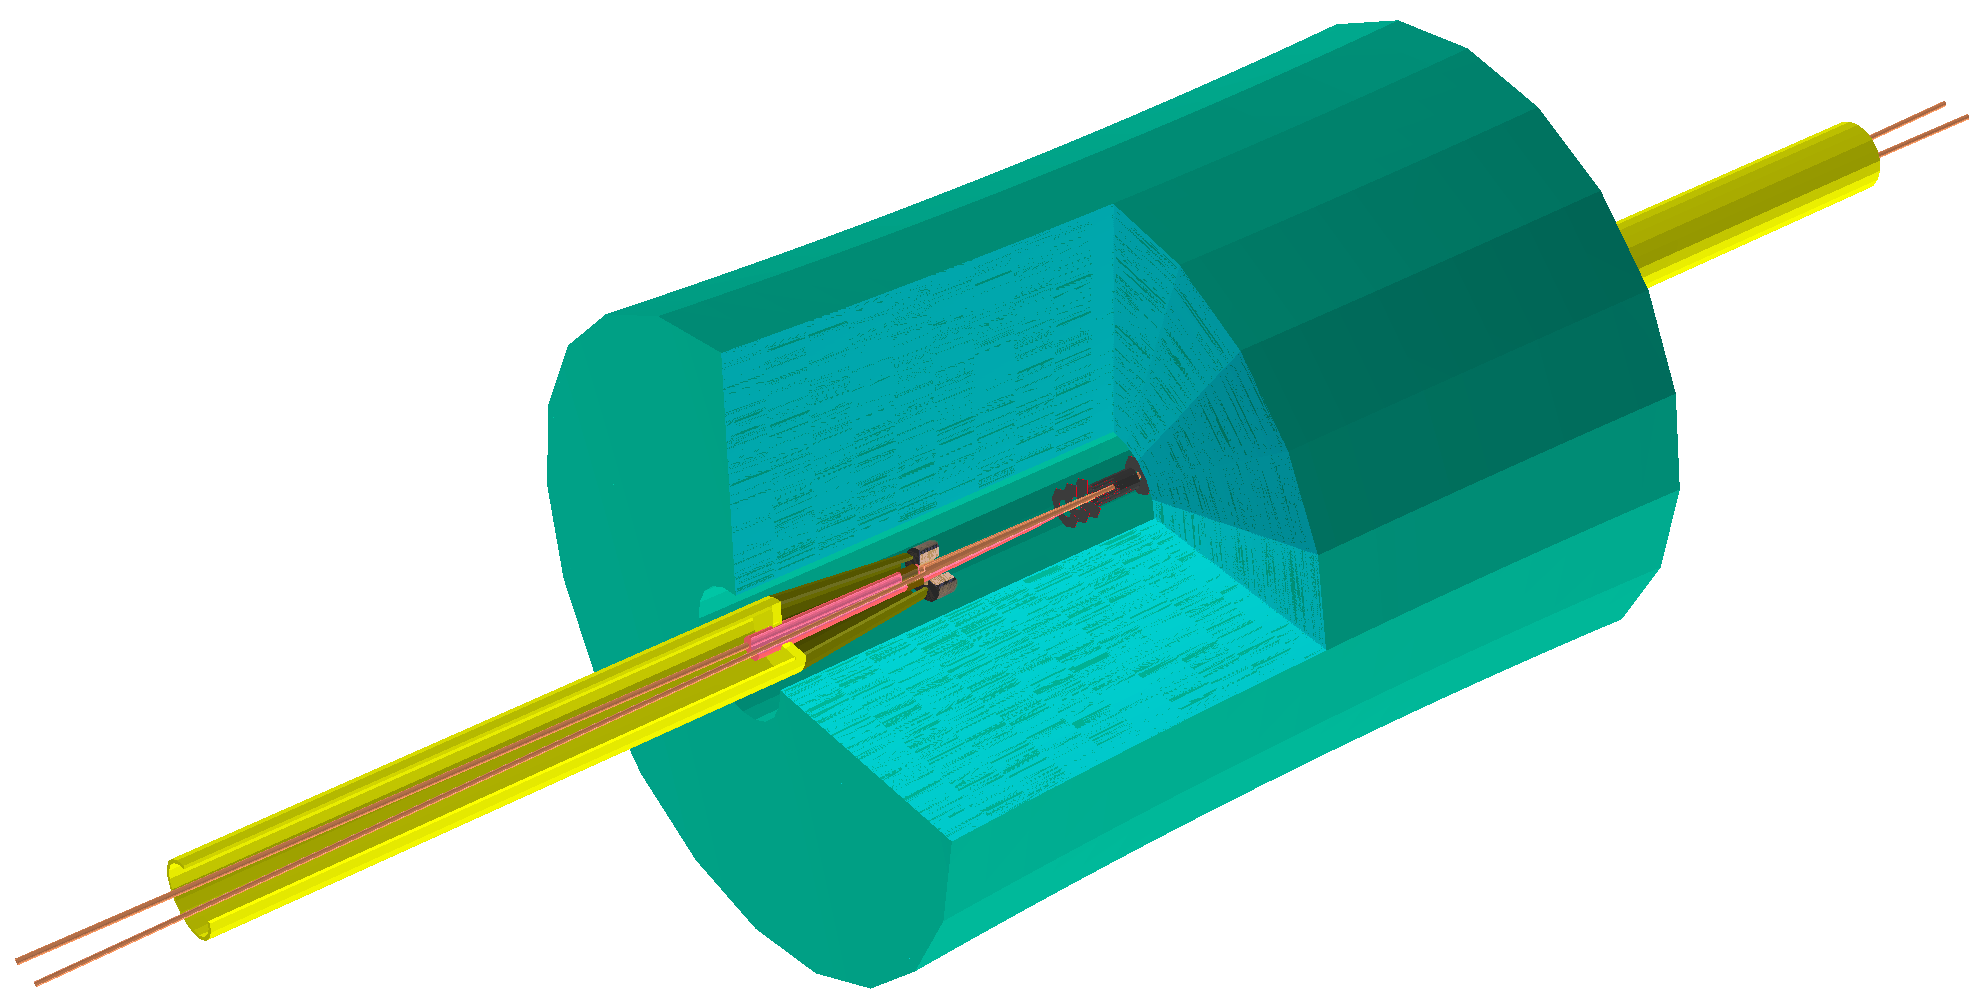
\includegraphics[width=\textwidth]{Figures/FCCeeIDEA_IR}};
    \begin{scope}[x={(image.south east)},y={(image.north west)}]

		% \draw[help lines,xstep=.1,ystep=.1] (0, 0) grid (1,1);
    %    \foreach \x in {0,1,...,9} { \node [anchor=north] at (\x/10,0) {0.\x}; }
    %    \foreach \y in {0,1,...,9} { \node [anchor=east] at (0,\y/10)
    %     {0.\y}; }


		\node[left] at (0.6, 0.7) {\textbf{Drift Chamber}};

		\draw[->, thick](0.05, 0.25) -- (0.05, 0.1);
		\node[above] at (0.05, 0.25) {\textbf{Beam Pipe}};

		\draw[->, thick](0.15, 0.45) -- (0.15, 0.22);
		\node[above] at (0.15, 0.45) {\textbf{Solenoid Shielding}};

		\draw[->, thick](0.2, 0.7) -- (0.42, 0.4);
		\node[above] at (0.2, 0.7) {\textbf{Tungsten Shielding}};

		\draw[->, thick](0.55, 0.05) -- (0.48, 0.4);
		\node[below] at (0.55, 0.05) {\textbf{Luminosity Calorimeter}};

		\draw[->, thick](0.75, 0.2) -- (0.58, 0.5);
		\node[below] at (0.75, 0.2) {\textbf{Vertex Detector}};

	\end{scope}
  \end{tikzpicture}

  % \column{0.5\textwidth}
  % \end{columns}


  \end{tcolorbox}
\end{textblock}

%%%%%%%%%%%%%%%%%%%%%%%%%%%%%%%%%%%%%
%%% Block %%%
%%%%%%%%%%%%%%%%%%%%%%%%%%%%%%%%%%%%%
\begin{textblock}{40}(0.5, 62)
  \begin{tcolorbox}[title=The simulation of the drift chamber \& coverage]

  \begin{columns}
    \column{0.5\textwidth}
      \begin{itemize}
        \item The first layer of the drift chamber
        \item Wires are illustrated using different colors
        \item The wires are rotated by a stereo angle to increase the hit resolution
      \end{itemize}
      \centering
      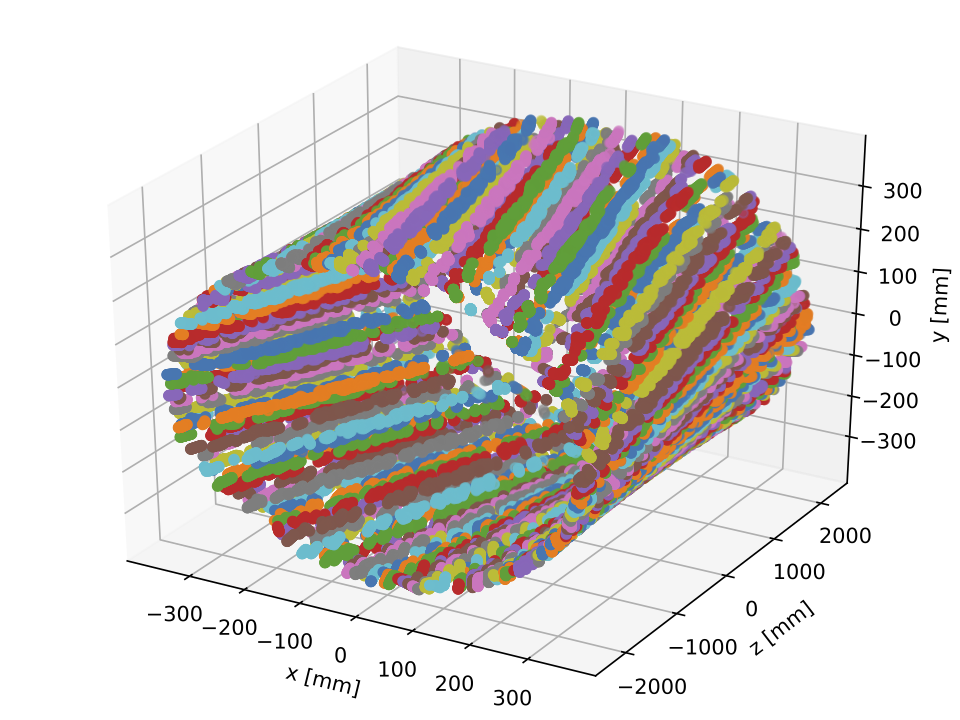
\includegraphics[width=\textwidth]{Figures/allHits}

    \column{0.5\textwidth}
      \begin{itemize}
        \item In the barrel region, the drift chamber has a high coverage of $\sim 112$ wires in average.
        \item In the forward region, silicon disks are foresean to increase the number of layers measuring the tracks.
      \end{itemize}
      \centering
      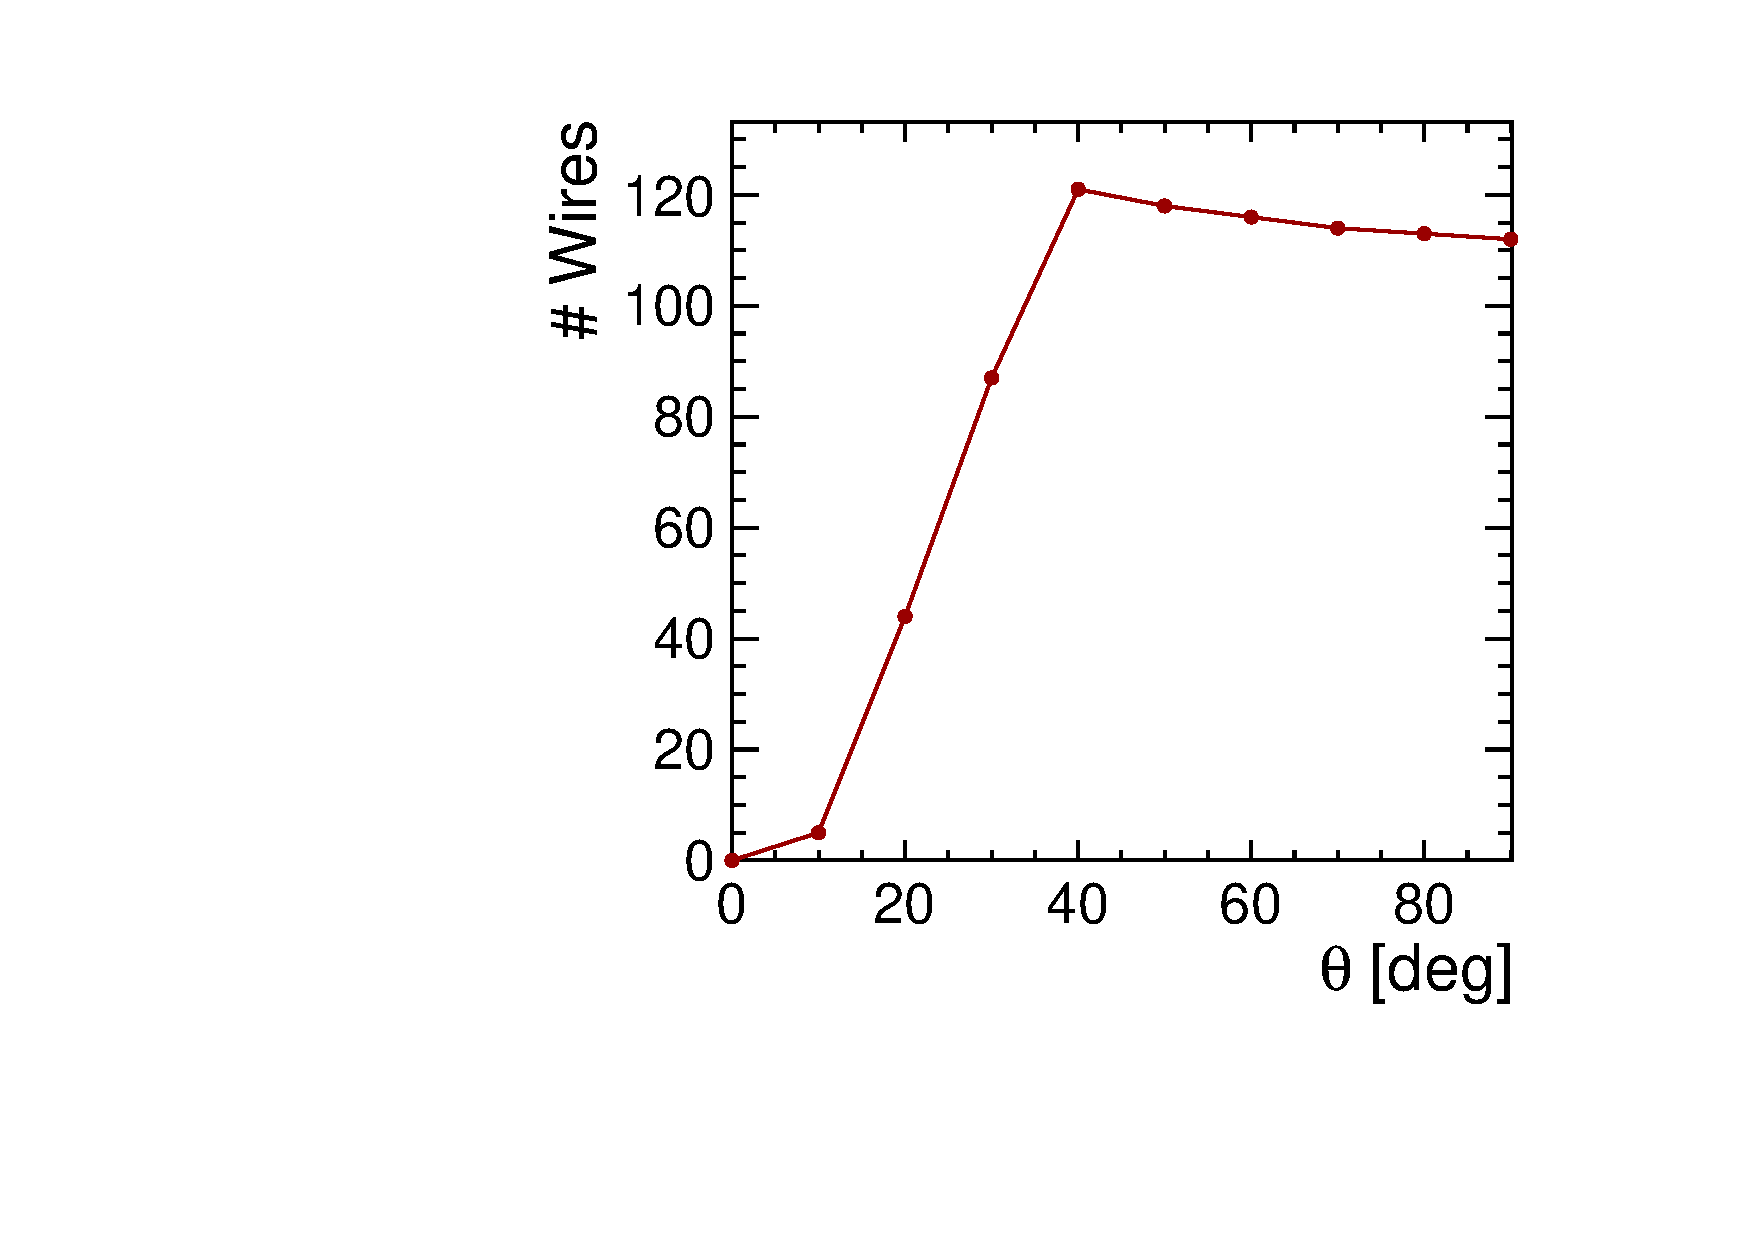
\includegraphics[width=\textwidth]{Figures/numWires}
  \end{columns}

  \end{tcolorbox}
\end{textblock}


%%%%%%%%%%%%%%%%%%%%%%%%%%%%%%%%%%%%%
%%% Block %%%
%%%%%%%%%%%%%%%%%%%%%%%%%%%%%%%%%%%%%
\begin{textblock}{40}(41, 55)
  \begin{tcolorbox}[title=Main sources of beam-induced backgrounds]

  \begin{columns}
    \column{0.5\textwidth}
    \begin{itemize}
      \item Three main sources of beam-induced backgrounds
      \begin{itemize}
        \item Incoherent $e^+e^-$ pairs du to bremstrahlung photons $\Rightarrow$ highest source of background
        \item $\gamma\gamma\rightarrow$ hadrons $\Rightarrow$ Expected to have a very low impact
        \item Synchrotron radiation (SR) $\Rightarrow$ Dictates the design of the interaction region (IR)
          \begin{itemize}
            \item Defines the beampipe radius, the design of the shielding (in Tungesten)
            \item Mostly stopped by the shielding, few SR photons can hit the detector
          \end{itemize}
      \end{itemize}
    \end{itemize}

    \column{0.5\textwidth}
    \begin{itemize}
      \item The trajectory of the $e^+e^−$ pairs in a 2~T magnetic field.
    \end{itemize}
    \centering
    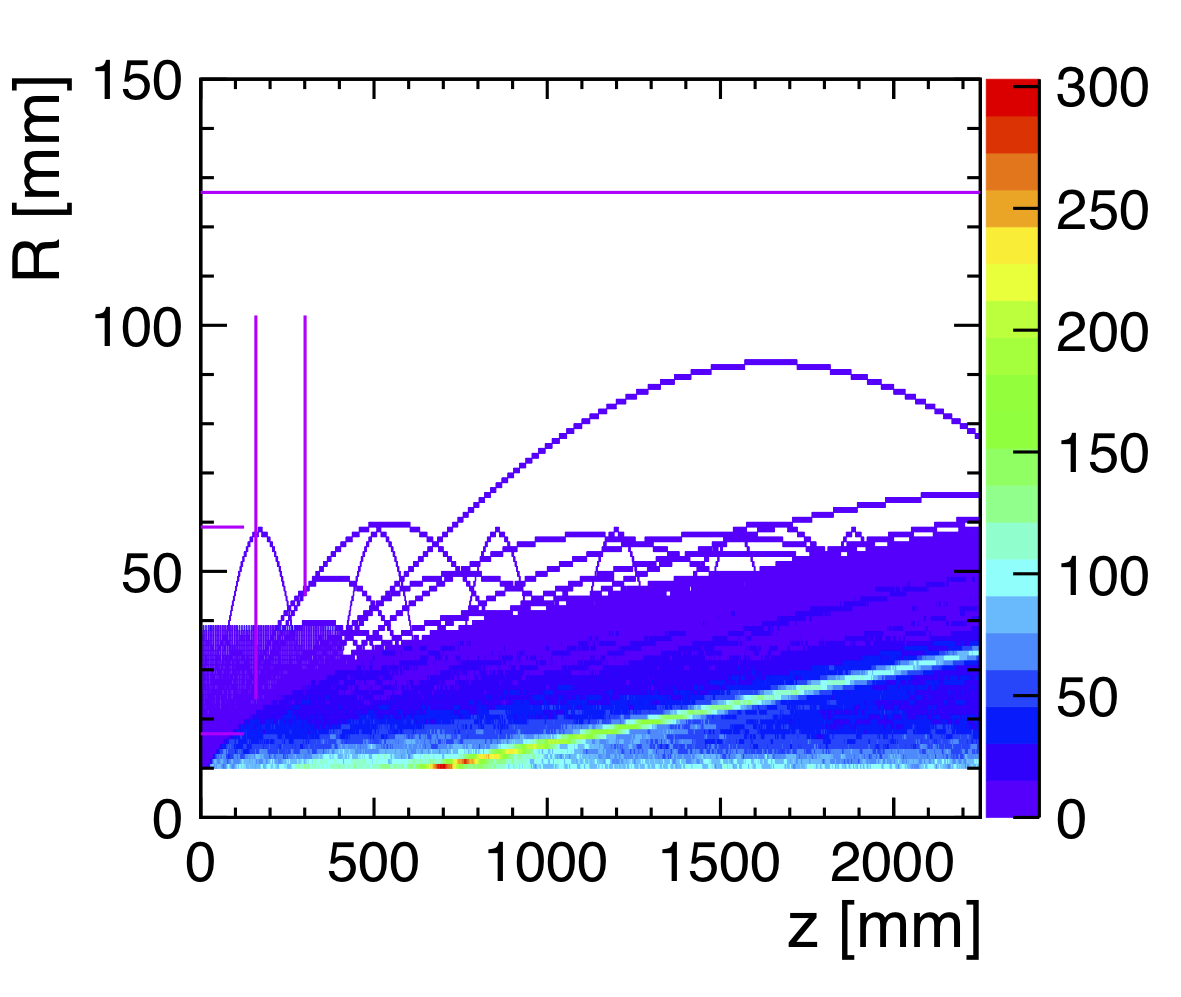
\includegraphics[width=\textwidth]{../figures/pairs_R_Z}
  \end{columns}

  \end{tcolorbox}
\end{textblock}

%%%%%%%%%%%%%%%%%%%%%%%%%%%%%%%%%%%%%
%%% Block %%%
%%%%%%%%%%%%%%%%%%%%%%%%%%%%%%%%%%%%%
\begin{textblock}{40}(41, 77)
  \begin{tcolorbox}[title=Summary of beam-induced backgrounds \& conclusions]

  \centering
	\begin{tabular}{l c c}
  	\toprule
	   Background & \multicolumn{2}{c}{Average occupancy} \\
	    & E\textsubscript{cm} = 91.2~GeV &  E\textsubscript{cm} = 365~GeV \\
	   \midrule
	   $e^+e^-$ pair background & 1.1\% & 2.9\% \\
	   $\gamma\gamma\rightarrow$ hadrons & 0.001\% & 0.035\%  \\
	   Synchrotron radiation & - & 0.2\% \\
	   \bottomrule
	\end{tabular}

  \begin{itemize}
    \item The overall impact remains low and the results are promising for the track reconstruction with this detector.
  \end{itemize}

  \end{tcolorbox}
\end{textblock}

%%%%%%%%%%%%%%%%%%%%%%%%%%%%%%%%%%%%%
%%% Block %%%
%%%%%%%%%%%%%%%%%%%%%%%%%%%%%%%%%%%%%
\begin{textblock}{80}(0.5, 90)
  \begin{tcolorbox}[title=3 main sources of beam-induced backgrounds at the top stage]

  \begin{columns}
    \column{0.33\textwidth}
    \begin{itemize}
      \item Incoherent $e^+e^-$ pairs
    \end{itemize}
    \centering
    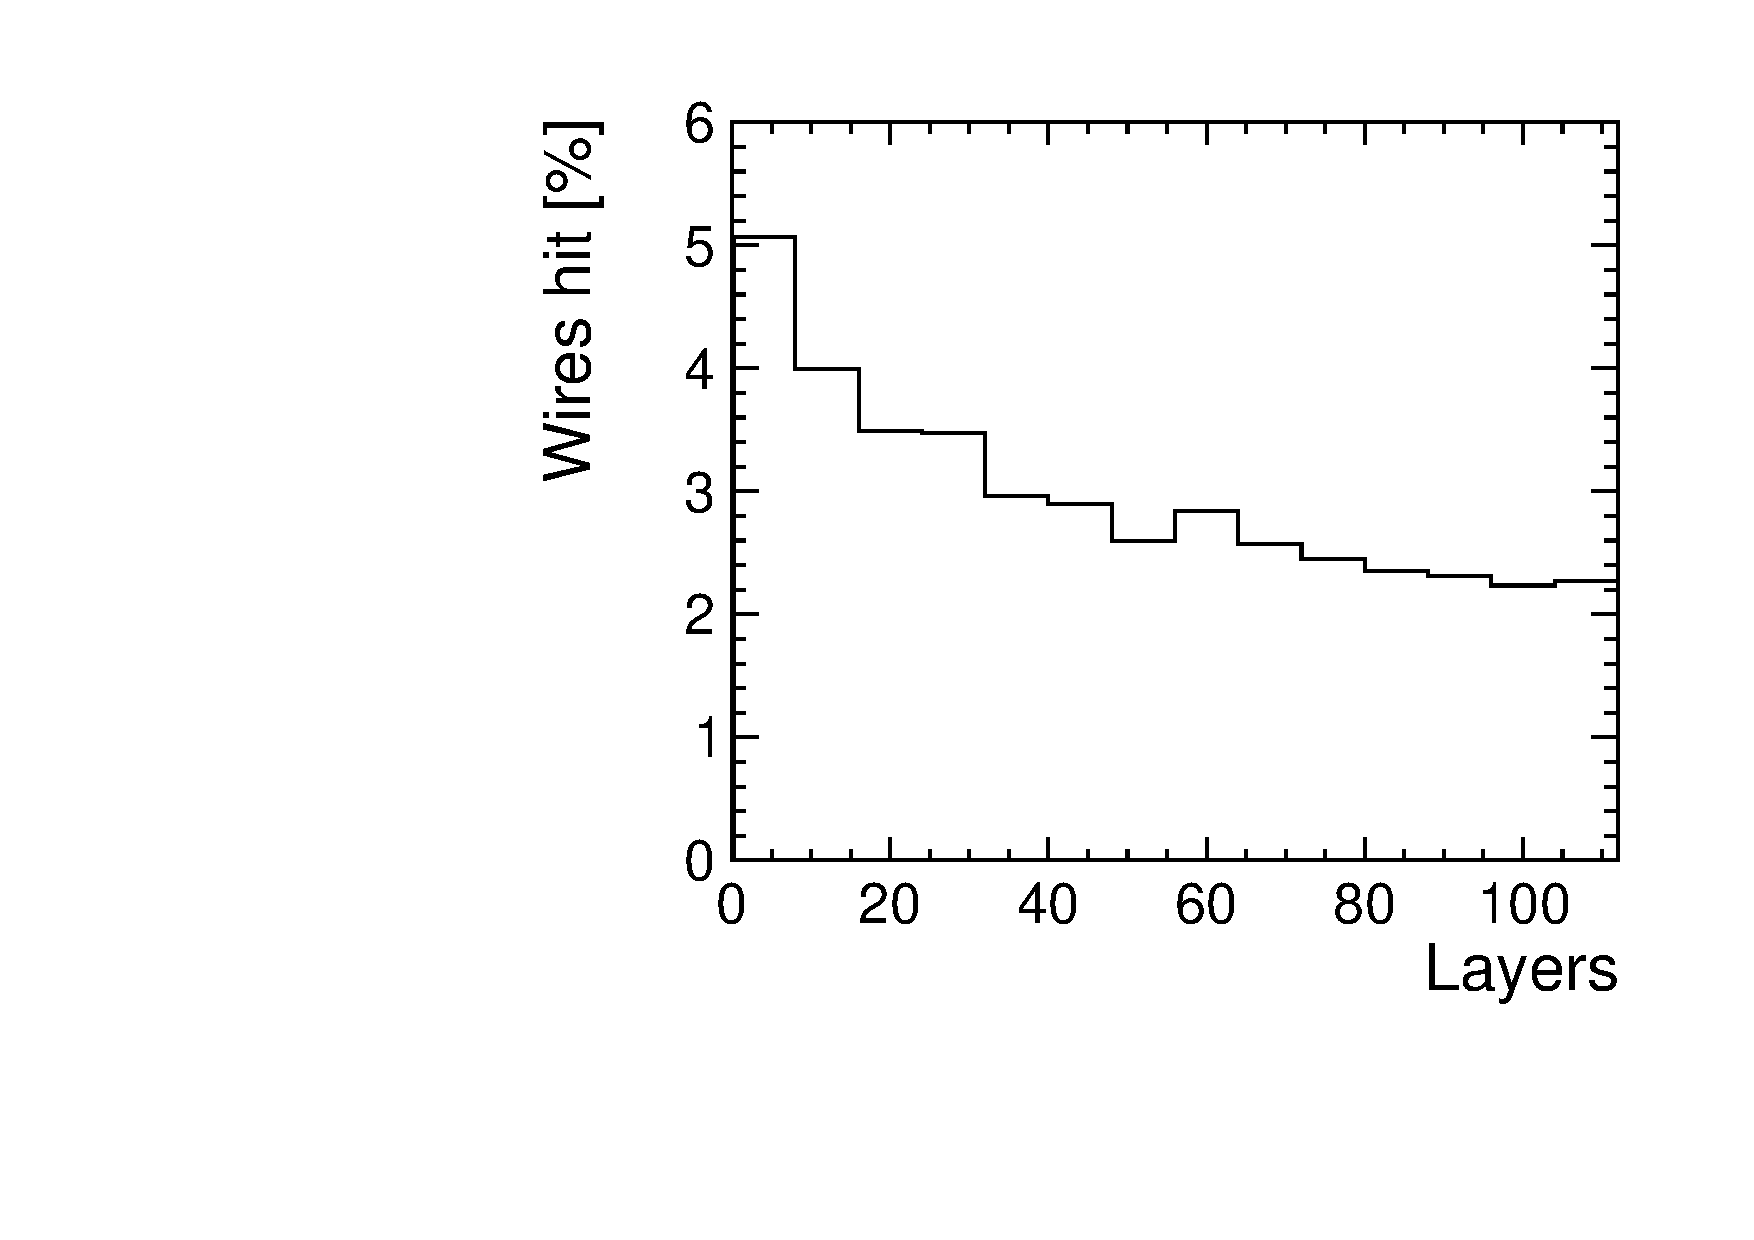
\includegraphics[width=\textwidth]{Figures/IPC_top}

    \column{0.33\textwidth}
    \begin{itemize}
      \item $\gamma\gamma\rightarrow$ hadrons
    \end{itemize}
    \centering
    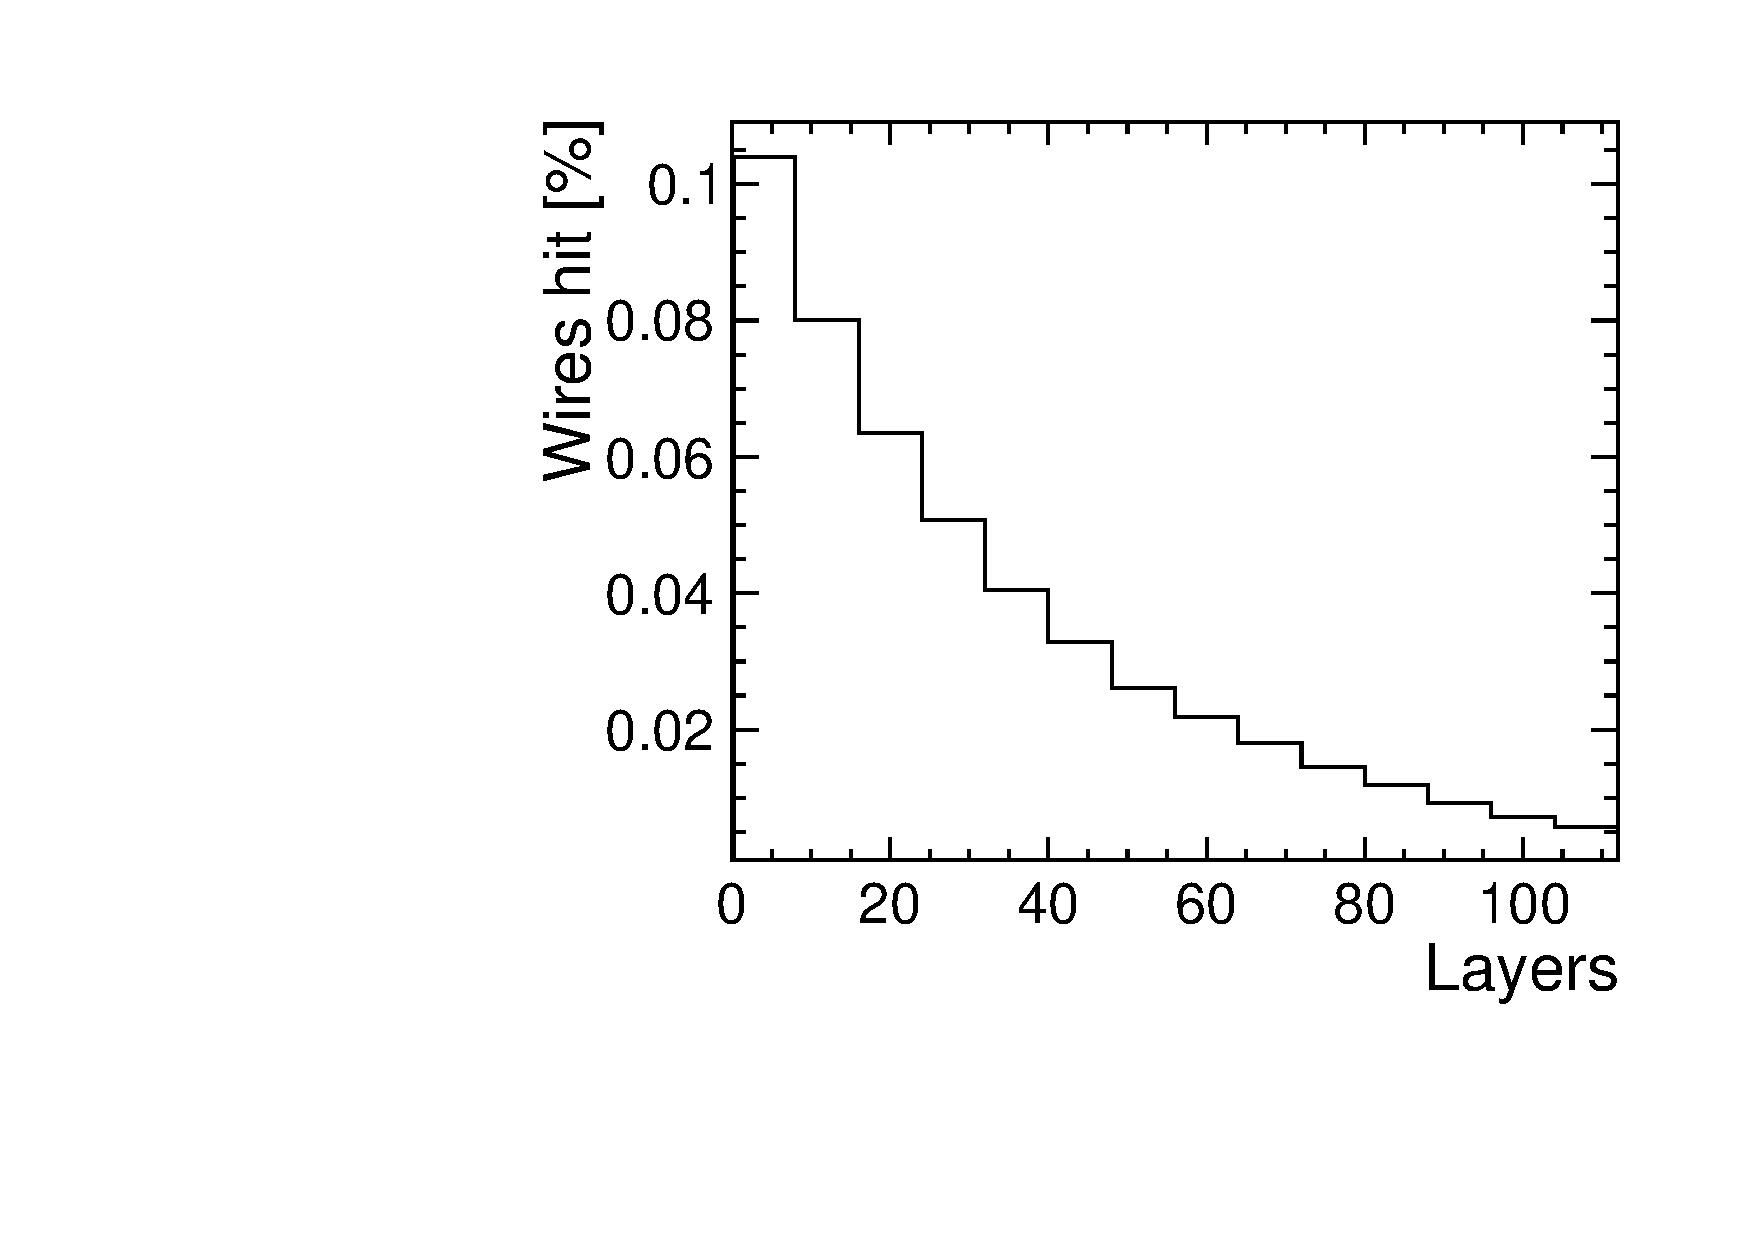
\includegraphics[width=\textwidth]{Figures/Hadrons_top}

    \column{0.33\textwidth}
    \begin{itemize}
      \item $\gamma\gamma\rightarrow$ hadrons
    \end{itemize}
    \centering
    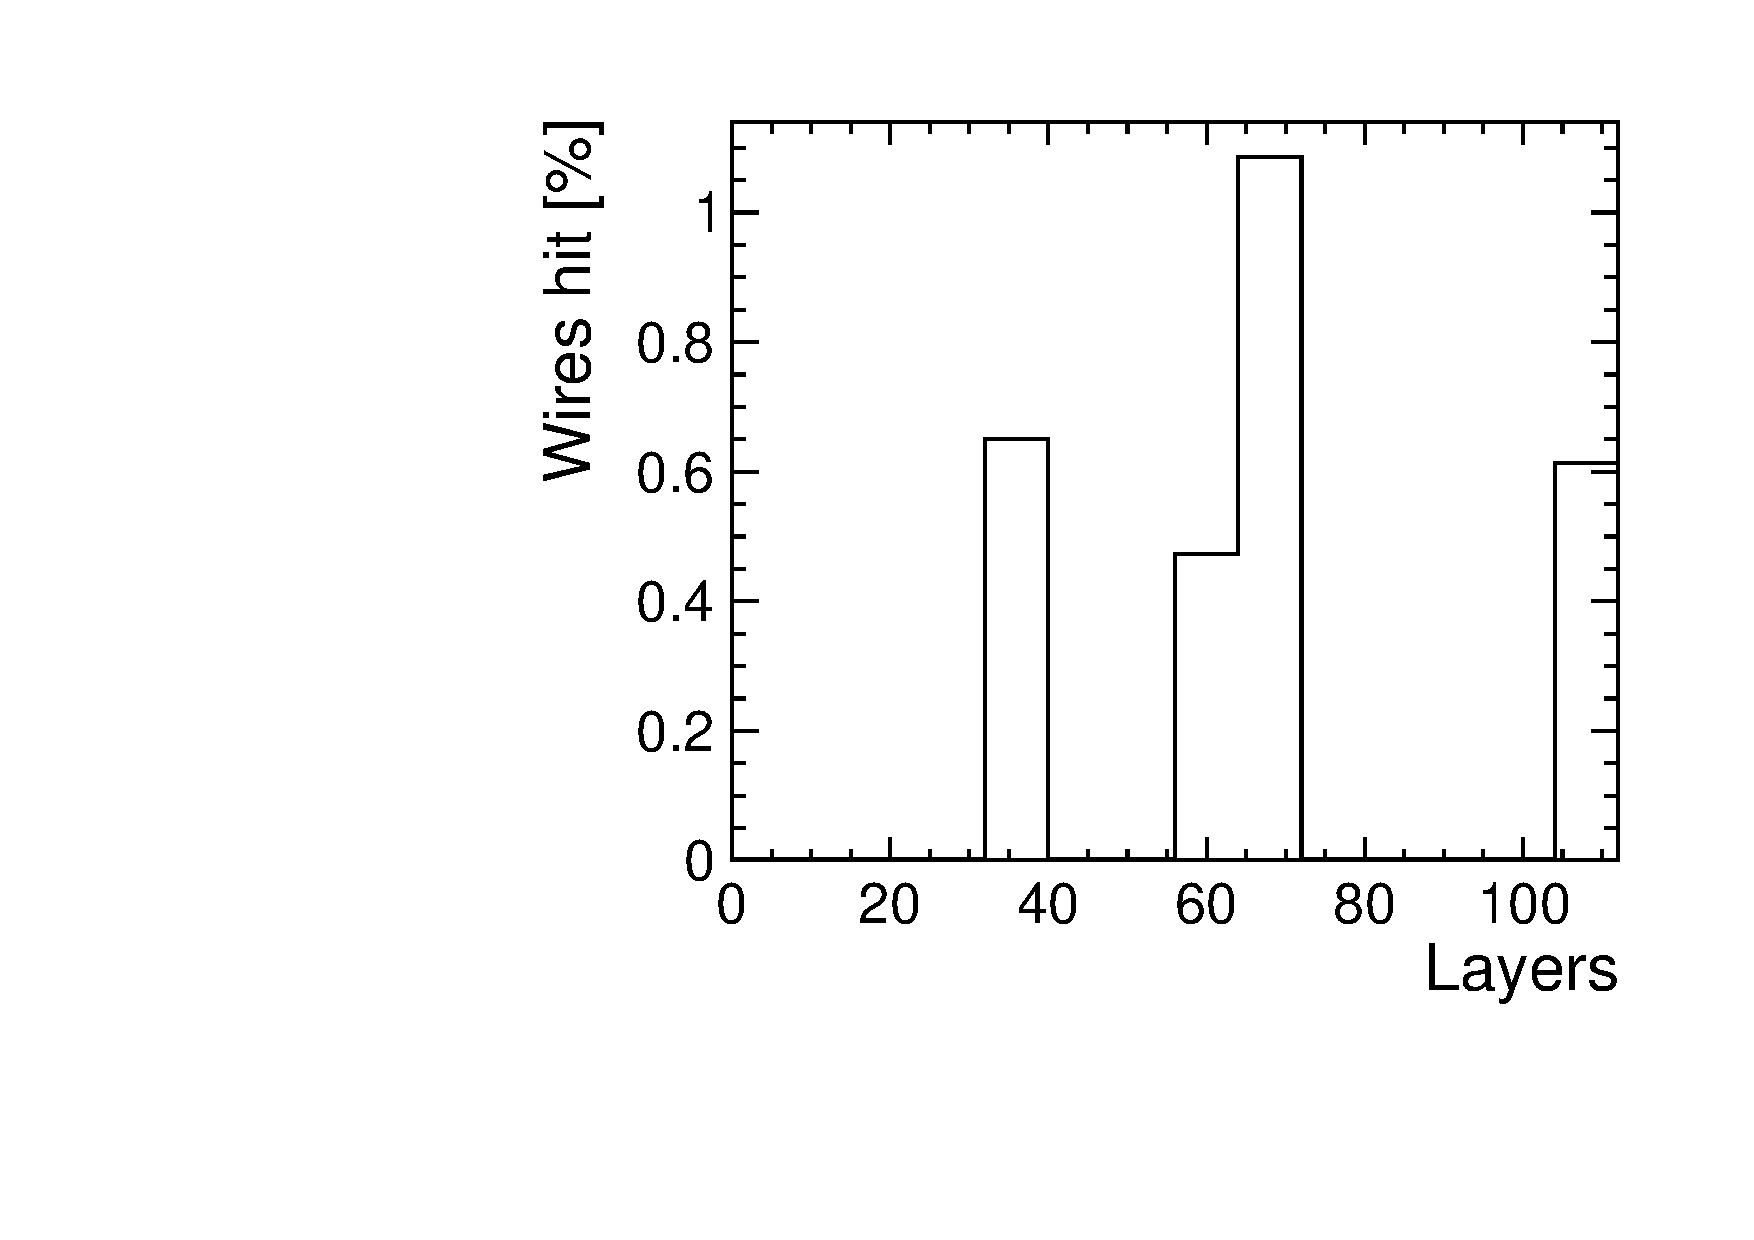
\includegraphics[width=\textwidth]{Figures/SR_top}

  \end{columns}

  \end{tcolorbox}
\end{textblock}

%--------------------------------------------%
\end{frame}
\end{document}
